\documentclass[portrait,a1paper,fontscale=0.46, margin = 5em, final]{baposter}

\usepackage[vlined]{algorithm2e}
\usepackage{times}
\usepackage{calc}
\usepackage{url}
\usepackage{graphicx}
\usepackage{subfig}
\usepackage{float}
\usepackage{amsmath}
\usepackage{amssymb}
\usepackage{relsize}
\usepackage{multirow}
\usepackage{booktabs}
\usepackage{multicol}
\usepackage[T1]{fontenc}
\usepackage{ae}
\usepackage{bm}
\usepackage{microtype}
\usepackage{pst-solides3d}

\graphicspath{{images/}}

 %%%%%%%%%%%%%%%%%%%%%%%%%%%%%%%%%%%%%%%%%%%%%%%%%%%%%%%%%%%%%%%%%%%%%%%%%%%%%%%%
 %%%% Some math symbols used in the text
 %%%%%%%%%%%%%%%%%%%%%%%%%%%%%%%%%%%%%%%%%%%%%%%%%%%%%%%%%%%%%%%%%%%%%%%%%%%%%%%%
 % Format
 \newcommand{\RotUP}[1]{\begin{sideways}#1\end{sideways}}
\newcommand{\ud}{\,\mathrm{d}}
\newcommand{\rulesep}{\unskip\ \vrule\ }
 %%%%%%%%%%%%%%%%%%%%%%%%%%%%%%%%%%%%%%%%%%%%%%%%%%%%%%%%%%%%%%%%%%%%%%%%%%%%%%%%
 % Multicol Settings
 %%%%%%%%%%%%%%%%%%%%%%%%%%%%%%%%%%%%%%%%%%%%%%%%%%%%%%%%%%%%%%%%%%%%%%%%%%%%%%%%
 \setlength{\columnsep}{0.7em}
 \setlength{\columnseprule}{0mm}


 %%%%%%%%%%%%%%%%%%%%%%%%%%%%%%%%%%%%%%%%%%%%%%%%%%%%%%%%%%%%%%%%%%%%%%%%%%%%%%%%
 % Save space in lists. Use this after the opening of the list
 %%%%%%%%%%%%%%%%%%%%%%%%%%%%%%%%%%%%%%%%%%%%%%%%%%%%%%%%%%%%%%%%%%%%%%%%%%%%%%%%
 \newcommand{\compresslist}{
 \setlength{\leftmargin}{0pt}
 \setlength{\itemsep}{0pt}
 \setlength{\parskip}{0pt}
 \setlength{\parsep}{0pt}
 }

%%%%%%%%%%%%%%%%%%%%%%%%%%%%%%%%%%%%%%%%%%%%%%%%%%%%%%%%%%%%%%%%%%%%%%%%%%%%%
%% Begin of Document
%%%%%%%%%%%%%%%%%%%%%%%%%%%%%%%%%%%%%%%%%%%%%%%%%%%%%%%%%%%%%%%%%%%%%%%%%%%%%
\begin{document}
%%%%%%%%%%%%%%%%%%%%%%%%%%%%%%%%%%%%%%%%%%%%%%%%%%%%%%%%%%%%%%%%%%%%%%%%%%%%%
%% Here starts the poster
%%---------------------------------------------------------------------------
%% Format it to your taste with the options
%%%%%%%%%%%%%%%%%%%%%%%%%%%%%%%%%%%%%%%%%%%%%%%%%%%%%%%%%%%%%%%%%%%%%%%%%%%%%
\begin{poster}{
 % Show grid to help with alignment
 grid=false,
 % Column spacing
 colspacing= 1em,
 columns=3,
 % backgroud color
 background=shadetb,
 bgColorTwo=black!5!white!90!,
 bgColorOne=white,
 % Color style
 headerColorOne=red!20!white!95!yellow,
 borderColor=red!50!white!95!yellow,
 % Format of textbox
 boxColorOne=white,
 textborder=rectangle,
 % Format of text header
 headerborder=open,
 headershape=roundedright,
 headershade=plain,
 headerheight=0.12\textheight}
 % university logo
 {
      \raisebox{0em}[5em][0em]{
\includegraphics[scale = 0.8]{GM-logo.png}}
 }
 % Title
 {\sc Spatio-temporal modelling for \\ \vspace{0.2em} global sea level change}
 % Author
 {\Large{Zhe Sha\textsuperscript{1},  Maike Schumancher\textsuperscript{1},  William Llovel\textsuperscript{1}, \\ 
 Jonathan Rougier\textsuperscript{2} and Jonathan Bamber\textsuperscript{1}
 \\
  \vspace{0.1em}
 {\textsuperscript{1}School of Geographical Sciences, University of Bristol \\
  \textsuperscript{2}School of Mathematics, University of Bristol}}\\
 \hspace{-3em} 
\noindent\makebox[\linewidth][c]{
\includegraphics[width = 1.1\paperwidth]{seplines}}
}
 % department logo
 {
  %\begin{tabular}{r}
    \raisebox{0em}[3em][0em]{
\includegraphics[scale = 0.23]{UoB-logo-colour.jpg}}
    %\raisebox{0em}[0em][0em]{\includegraphics[height=0.03\textheight]{oulogo}}
  %\end{tabular}

 }


%%%%%%%%%%%%%%%%%%%%%%%%%%%%%%%%%%%%%%%%%%%%%%%%%%%%%%%%%%%%%%%%%%%%%%%%%%%%%%
%%% Now define the boxes that make up the poster
%%%---------------------------------------------------------------------------
%%% Each box has a name and can be placed absolutely or relatively.
%%% The only inconvenience is that you can only specify a relative position
%%% towards an already declared box. So if you have a box attached to the
%%% bottom, one to the top and a third one which should be inbetween, you
%%% have to specify the top and bottom boxes before you specify the middle
%%% box.
%%%%%%%%%%%%%%%%%%%%%%%%%%%%%%%%%%%%%%%%%%%%%%%%%%%%%%%%%%%%%%%%%%%%%%%%%%%%%%

%%%%%%%%%%%%%%%%%%%%%%%%%%%%%%%%%%%%%%%%%%%%%%%%%%%%%%%%%%%%%%%%%%%%%%%%%%%%%%
  \headerbox{1. Introduction and framework}{name=intro,column=0,row=0, span = 3}{
  \begin{minipage}{0.25\textwidth}
 \textbf{Motivation}
  
Future sea level rise (SLR) is one of the most serious consequences of climate change. Traditionally, the Earth system components, including oceans, land ice, terrestrial water storage, and solid Earth effects, that contribute to SLR were treated separately and often led to inconsistencies between discipline-specific estimates of each part of the sea level budget.

\vspace{1.5em}
Our project aims at producing a physically-based, data-driven solution for the complete coupled land-ocean-solid Earth system that is consistent with the full suite of observations, prior knowledge and fundamental geophysical constraints.
  \end{minipage}
 \begin{minipage}{0.4\textwidth}
 \begin{figure}[H]
\centering
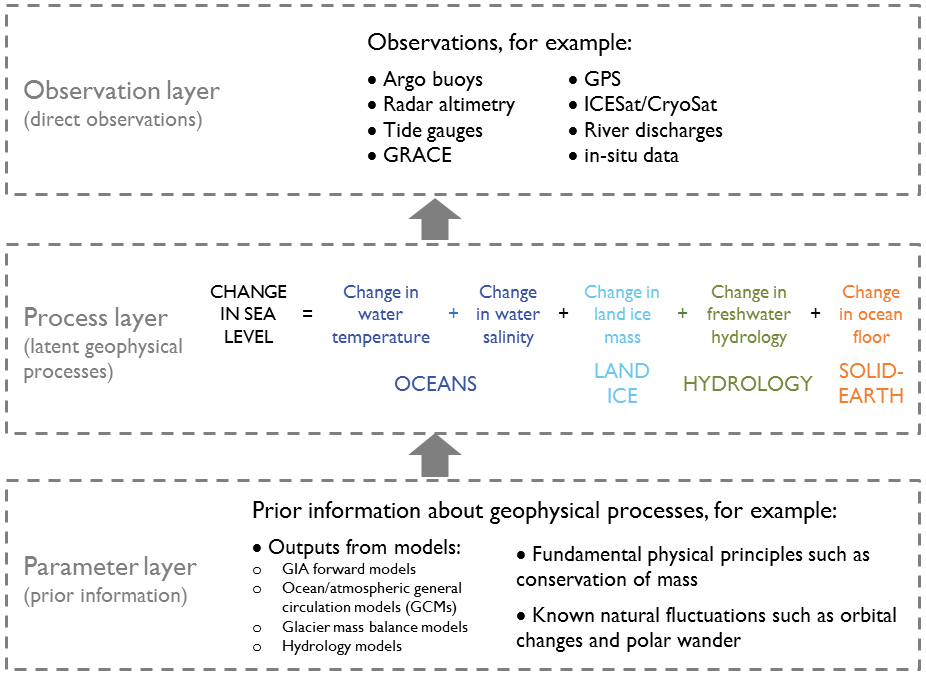
\includegraphics[width = 0.85\textwidth]{GMconcept-simplified}
\caption{Global Mass concept and framework.}
\end{figure}
 \end{minipage}
\begin{minipage}{0.34\textwidth}
\begin{center}
\textbf{Bayesian Hierarchical Model (BHM) }\cite{AZM2015}
\end{center}
Define $\bm{y}$ as the observations, $\bm{x}$ the latent process at the spatial unit of $\bm{y}$, $\bm{X}$ the latent process, and $\bm{\beta}$ and $\bm{\theta}$ the parameters to be estimated. 
\begin{align*}
\bm{y} | \bm{\beta}, \bm{x}, \bm{\theta} &\sim \mathcal{N}(\bm{P}(\bm{\beta}) \bm{x}, \bm{\Sigma_{obs}}), \\
\bm{x} | \mathcal{A}, \bm{X}, \bm{\theta} &\sim \mathcal{N}(\mathcal{A}\bm{X}, \bm{Q}^{-1}(\bm{\theta})),\\
\bm{X(\bm{s})} | \bm{\theta}, &\sim \mathcal{GP} (\bm{\mu}(\bm{s}), k(\bm{s}, \bm{r}; \bm{\theta})), \\
\bm{\beta} &\sim \mathcal{N}(\bm{\mu}_{\bm{\beta}}, \bm{\Sigma}_{\bm{\beta}}),\\
f(\bm{\theta}) &\sim \mathcal{N}(\bm{\mu}_{\bm{\theta}}, \bm{\Sigma}_{\bm{\theta}}).
\end{align*}
where $\bm{P}$ maps the latent process to  the observations, $\bm{\Sigma_{obs}}$ is a given measurement error matrix, $\mathcal{A}$ maps $\bm{X}$ into the spatial unit of $\bm{y}$, $\bm{Q}$ is a sparse precision matrix given by the stochastic partial differential equation (SPDE) approach \cite{SPDE}.
\end{minipage}
}
%%%%%%%%%%%%%%%%%%%%%%%%%%%%%%%%%%%%%%%%%%%%%%%%%%%%%%%%%%%%%%%%%%%%%%%%%%%%%%
  \headerbox{2. Big data challenges}{name=data,column=0,span = 3, below = intro }{
 \begin{minipage}{0.35\textwidth}
\begin{figure}[H]
\centering
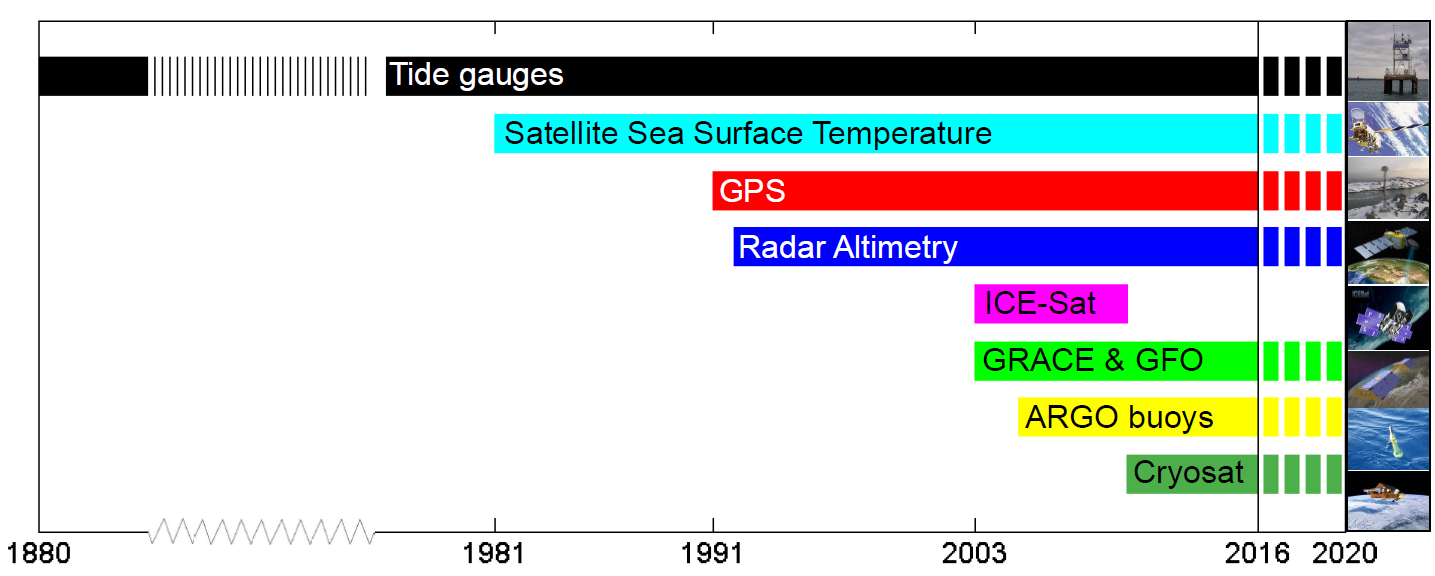
\includegraphics[width =\textwidth]{data}
\caption{Temporal coverage of the observations.}
\end{figure}

\textbf{Challenges}

\begin{itemize}\compresslist
\item Massive volume of data sets with uncertainty in error estimates.
\item Inconsistent temporal coverages and frequencies between the data sets.
\item In-situ and satellite measurements exhibit various spatial footprints.
\item Different spatially-varying mesh grids in high resolutions for SPDE approximation.
\end{itemize}

\textbf{Example: Glacio-Isostatic Adjustment (GIA)}

GIA describes the ongoing movement of land once burdened by ice-age glaciers and makes a crucial contribution to sea level rise evaluation.
\end{minipage}
\begin{minipage}{0.65\textwidth}
\begin{figure}[H]
\centering
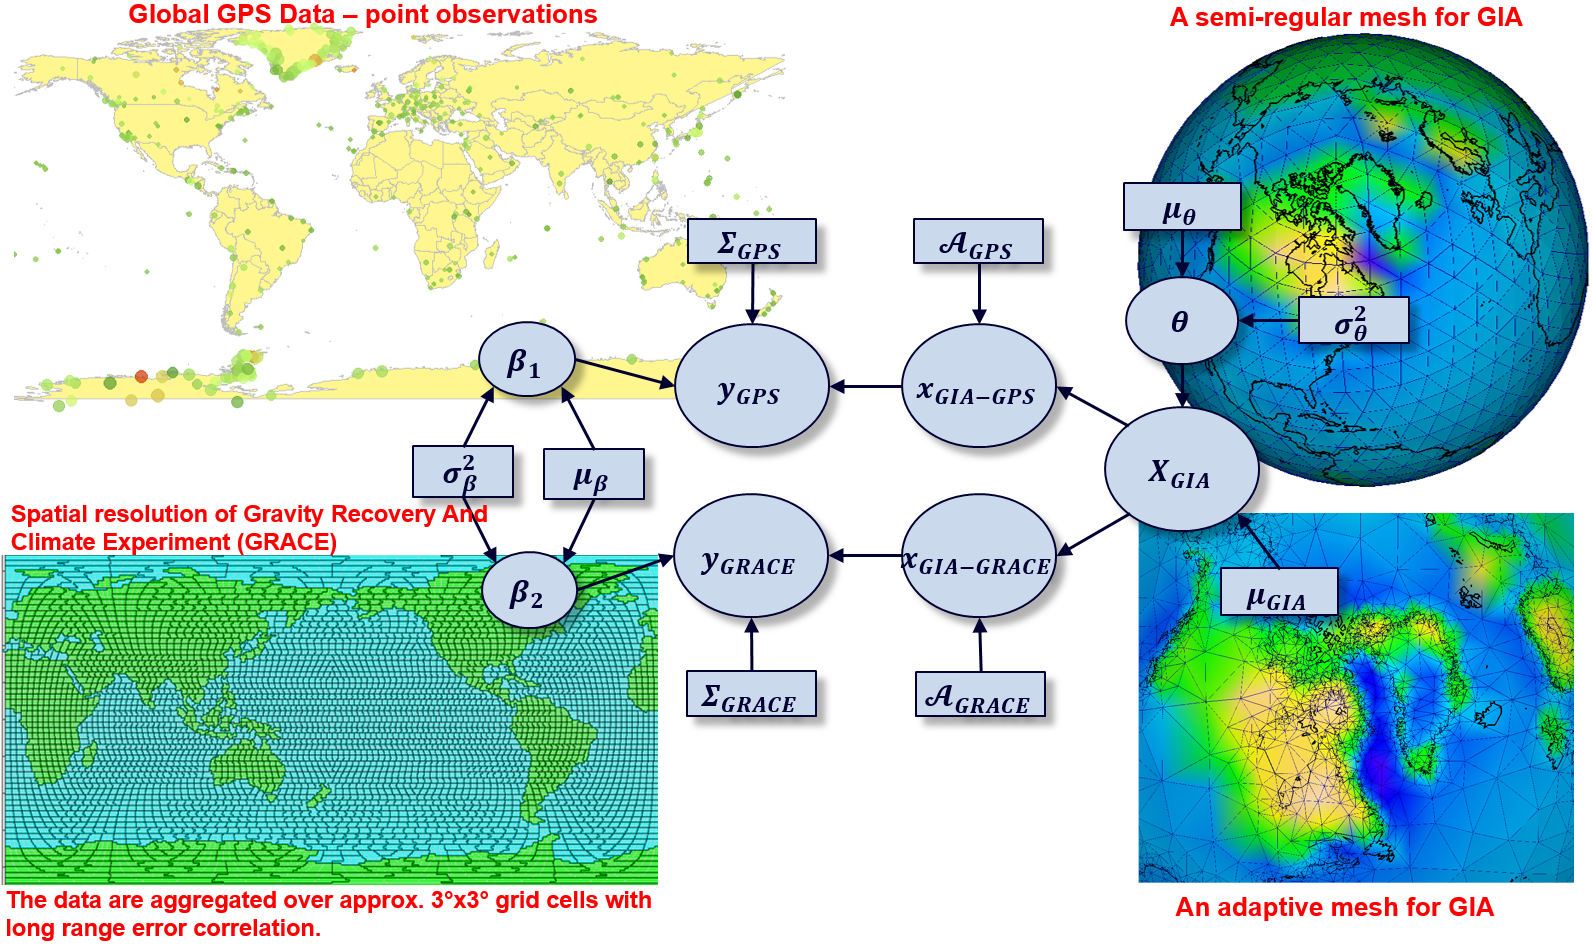
\includegraphics[width = 0.95\textwidth]{GIA}
\caption{The data sets, meshes and graphical model for GIA.}
\end{figure}
\end{minipage}
  }
  %%%%%%%%%%%%%%%%%%%%%%%%%%%%%%%%%%%%%%%%%%%%%%%%%%%%%%%%%%%%%%%%%%%%%%%%%%%%%%
\headerbox{3. Initial solution for the GIA process}{name=result,column = 0, span = 2,
 below = data}{
 \begin{minipage}{0.28\textwidth}
Initial GIA solution combines global GPS data and prior means from a physical forward model, using a semi-regular mesh on a sphere at approximately 10 degree resolution.
 
Right shows the predicted GIA mean field. The predicted errors at the GPS locations and a set of regular grid points are shown as blue disks with disk radius proportional to the error size. 
 
 The data present strong signals at the GPS locations with much smaller predicted errors than elsewhere.
 \end{minipage}
\begin{minipage}{0.72\textwidth}
\begin{figure}[H]
\centering
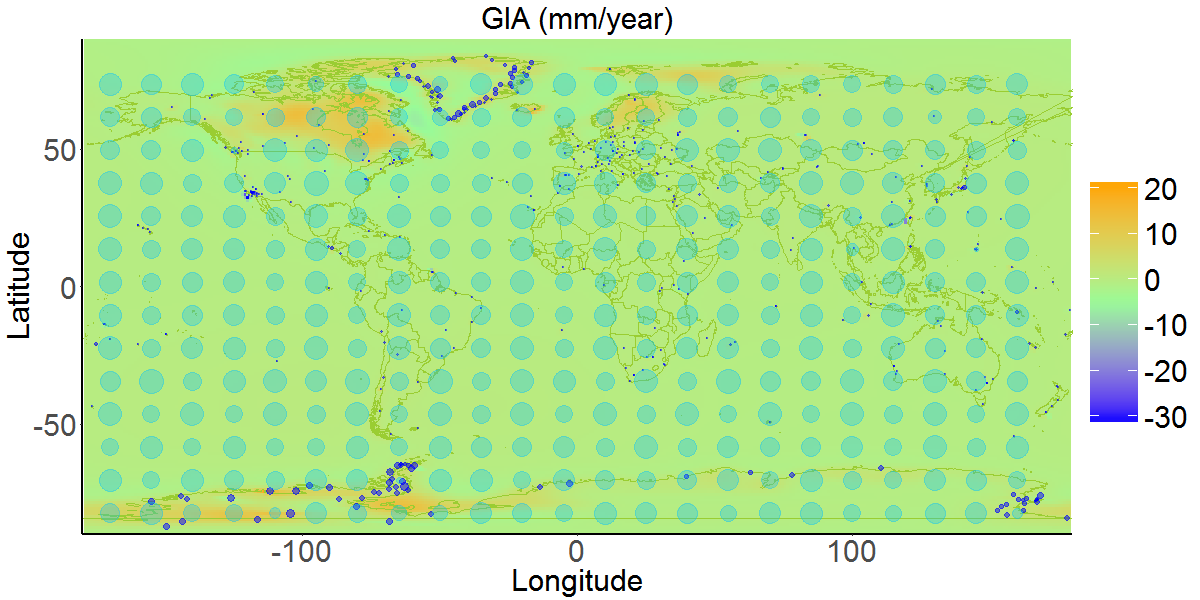
\includegraphics[width = \textwidth]{GIA_map}
\caption{Predicted GIA mean field.}\label{fig:GIA}
\end{figure}
\end{minipage}
 }

  %%%%%%%%%%%%%%%%%%%%%%%%%%%%%%%%%%%%%%%%%%%%%%%%%%%%%%%%%%%%%%%%%%%%%%%%%%%%%%
  \headerbox{4. Future Work}{name=future,column=0, span = 2, below = result}{
\begin{itemize}\compresslist
\item Integrating flexible temporal structure into the multivariate processes.
\item Improving mesh quality and resolution.
\item Estimating a data-driven GIA solution based on the full framework.
\item Closing the sea level budget for the last four decades by adding physical constraints and more datasets.
\end{itemize}

  }
   %%%%%%%%%%%%%%%%%%%%%%%%%%%%%%%%%%%%%%%%%%%%%%%%%%%%%%%%%%%%%%%%%%%%%%%%%%%%%%
\headerbox{Acknowledgements}{name=ack,column=2,below=data}{
\small{Funded by the European Research Council (ERC) under the European Union's Horizon 2020 research and innovation programme under grant agreement No 69418.}
\begin{figure}[H]
  \centering
  \begin{tabular}{c|c}
    \subfloat{
\includegraphics[width = 0.25\textwidth]{EUflag}} \hspace{2em} &
    \hspace{2em} \subfloat{
\includegraphics[width = 0.25\textwidth]{ERClogo}}
  \end{tabular}
\end{figure}


}
 %%%%%%%%%%%%%%%%%%%%%%%%%%%%%%%%%%%%%%%%%%%%%%%%%%%%%%%%%%%%%%%%%%%%%%%%%%%%%%
\headerbox{Keep in touch}{name=contact,column=2,below=ack}{
Website: www.globalmass.eu 

Email: globalmass-project@bristol.ac.uk

Follow us on Twitter: @GlobalMassTeam

  }
  
  %%%%%%%%%%%%%%%%%%%%%%%%%%%%%%%%%%%%%%%%%%%%%%%%%%%%%%%%%%%%%%%%%%%%%%%%%%%%%%


\headerbox{References}{name=ref,column=2,  below=contact}{

\renewcommand{\refname}{\vspace{-1em}}
\bibliographystyle{abbrv}
\footnotesize{\bibliography{references}}

  }
 
\end{poster}

\end{document}
